\documentclass[13pt,oneside]{book}
\usepackage[utf8]{inputenc}
\usepackage{url}
\usepackage{graphicx}

\usepackage{geometry}
\geometry{a4paper, left=20mm, right=20mm, top=20mm, bottom=20mm}
\usepackage[margin=1.2in]{geometry}
\usepackage[toc,page]{appendix}
\usepackage{graphicx}
\usepackage{natbib}
\usepackage{lipsum}
\usepackage{caption}

\begin{document}

\captionsetup[figure]{margin=1.5cm,font=small,labelfont={bf},name={Figure},labelsep=colon,textfont={it}}
\captionsetup[table]{margin=1.5cm,font=small,labelfont={bf},name={Table},labelsep=colon,textfont={it}}
\setlipsumdefault{1}

\begin{titlepage}
\begin{center}
{\LARGE College Of Engineering Trivandrum}\\[3cm]
\linespread{1.2}\huge {\bfseries Application Software Development Lab}\\[3cm]
\linespread{1}

\includegraphics[width=5cm]{img/emblem.jpeg}\\[3cm]
{\Large GOKUL K\\ S5  CSE \\ Roll No:21\\ TVE18CS021 }\\[1cm]


\textit{ }\\[2cm]
Department of Computer Science\\[0.2cm]
\today
\end{center}

\end{titlepage}

\newpage

\begin{frame}{}
    \centering
    \hspace*{-0.5cm}
    $\vcenter{\hbox{
\includegraphics[width=1.5cm]{img/emblem.jpeg}}}$
    $\vcenter{\resizebox{0.95\textwidth}{!}{
        \begin{tabular}{c}
             CS333 - Application Software Development Lab $\cdot$ 2020 $\cdot$   \\
             \hline 
        \end{tabular}
    }}$
\end{frame}
\section*{Cycle 2}
\section*{Expt 1}
\begin{center}
    \Large{PL/SQL AND SEQUENCE}
\end{center}

\section*{Aim}
\large To study the basic PL/SQL and sequence queries.
\section*{Expiriment}
\begin{itemize}
\item
To print the first `n' prime numbers.
 
 
Syntax:
\begin{verbatim}
CREATE OR REPLACE FUNCTION prime(N int) RETURNS VOID AS $$
DECLARE
        flag INT;
        count INT = 0;
        i INT;
        counter INT = 2;
        remainder INT;
BEGIN
        WHILE (count < N) LOOP
                flag = 0;
                FOR i IN 2..(counter/2) LOOP
                        remainder = counter % i;
                        IF remainder = 0 THEN
                                flag = 1;
                        END IF;
                END LOOP;
                IF flag = 0 THEN
                        RAISE NOTICE '%', counter;
                        count = count + 1;
                END IF;
                counter = counter+1;
        END LOOP;
END;
$$ LANGUAGE plpgsql;

\end{verbatim}
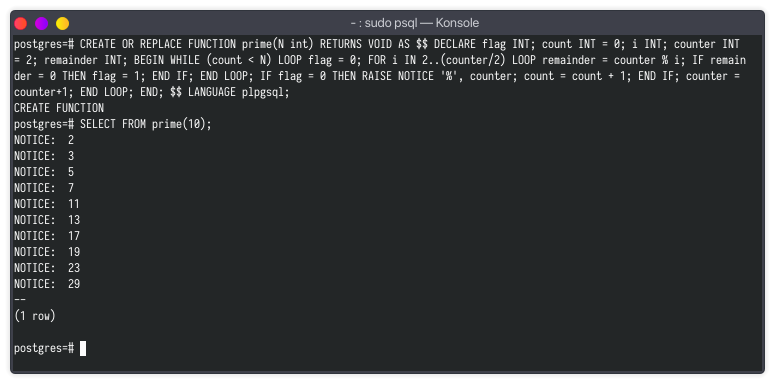
\includegraphics[width=0.9\textwidth]{img/p8/ss1.png}


\item
Display the Fibonacci series up to `n' terms.
 
 
Syntax:
\begin{verbatim}
CREATE OR REPLACE FUNCTION fib(N int) RETURNS VOID AS $$ 
DECLARE
        temp INT = 0;
        a INT = 1;
        b INT = 0;
        count INT = 0;
BEGIN
        WHILE (count < N) LOOP
                RAISE NOTICE '%', a;
                temp = a;
                a = a+b;
                b = temp;
                count = count+1;
        END LOOP;
END;
$$ LANGUAGE plpgsql;

\end{verbatim}
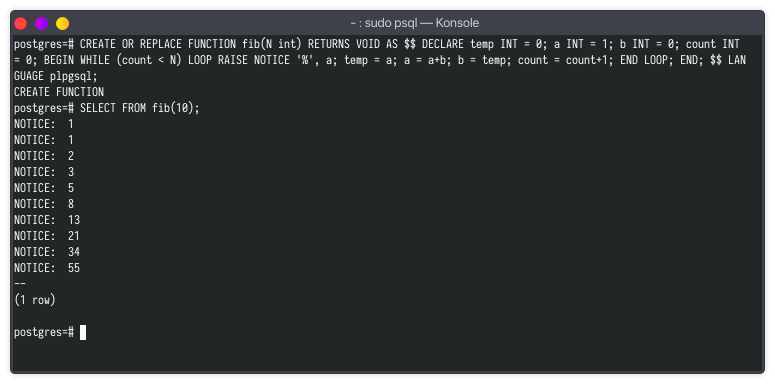
\includegraphics[width=0.9\textwidth]{img/p8/ss2.png}


\item
Create a table named student grade with the given attributes:
 roll, name, mark1, mark2, mark3, grade. Read the roll, name and marks from the user.
 Calculate the grade of the student and insert a tuple into the table using PL/SQL.
 (Grade= `PASS' if AVG >40, Grade='FAIL' otherwise)
 
 
Syntax:
\begin{verbatim}
CREATE TABLE IF NOT EXISTS StudentGrade (
        rollno INT,
        name VARCHAR(20),
        mark1 INT,
        mark2 INT,
        mark3 INT,
        status VARCHAR(4)
);
CREATE OR REPLACE FUNCTION read_marks(
        rollno INT,
        name VARCHAR(20),
        mark1 INT,
        mark2 INT,
        mark3 INT
) RETURNS VOID AS $$
DECLARE
        status VARCHAR(4);
BEGIN
        IF ((mark1 + mark2 +mark3)/3 > 40) THEN
                status = 'PASS';
        ELSE 
                status = 'FAIL';
        END IF;
        INSERT INTO StudentGrade VALUES (rollno, name, mark1, mark2, mark3, status);
END;
$$ LANGUAGE plpgsql;

\end{verbatim}
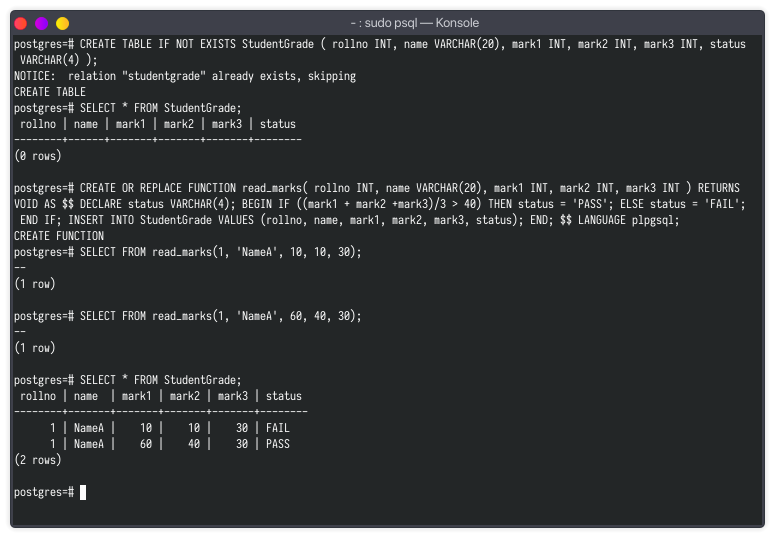
\includegraphics[width=0.9\textwidth]{img/p8/ss3.png}


\item
Create table circle\_area (rad, area). For radius 5,10,15,20 and 2. Find the area and
insert the corresponding values into the table by using loop structure in PL/SQL.
Syntax:
\begin{verbatim}
CREATE TABLE IF NOT EXISTS circle_area (
        rad INT,
        area DECIMAL(10, 2)
);
CREATE OR REPLACE FUNCTION find_area() RETURNS VOID AS $$
DECLARE
        area INT;
        rad_array INT[] := ARRAY[5, 10, 15, 20, 25];
        rad INT;
BEGIN
        FOREACH rad IN ARRAY rad_array LOOP
                INSERT INTO circle_area VALUES 
                        (rad, 3.14*rad*rad);
        END LOOP;
END;
$$ LANGUAGE plpgsql;

\end{verbatim}
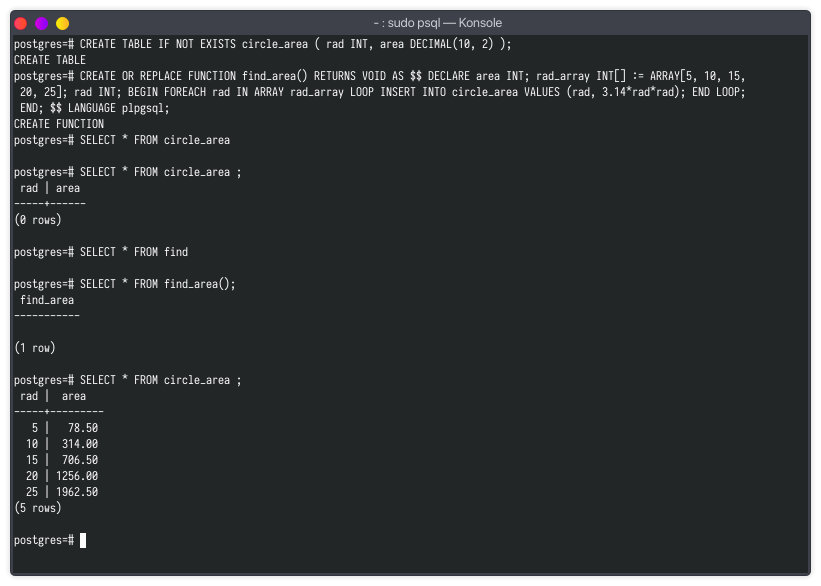
\includegraphics[width=0.9\textwidth]{img/p8/ss4.png}


\item 
 5. Use an array to store the names, marks of 10 students in a class. Using Loop
 structures in PL/SQL insert the ten tuples to a table named student.
 
 
Syntax:
\begin{verbatim}
CREATE TABLE IF NOT EXISTS student (
        name VARCHAR(20),
        marks INT
);
CREATE OR REPLACE FUNCTION insert_marks() RETURNS VOID AS $$
DECLARE
        names VARCHAR(20)[] := ARRAY['Name1', 'Name2', 'Name3'];
        marks INT[] := ARRAY[10, 20, 40];
BEGIN
        FOR i IN 1..3 LOOP
                INSERT INTO student VALUES (names[i], marks[i]);
        END LOOP;
END;
$$ LANGUAGE plpgsql;

\end{verbatim}
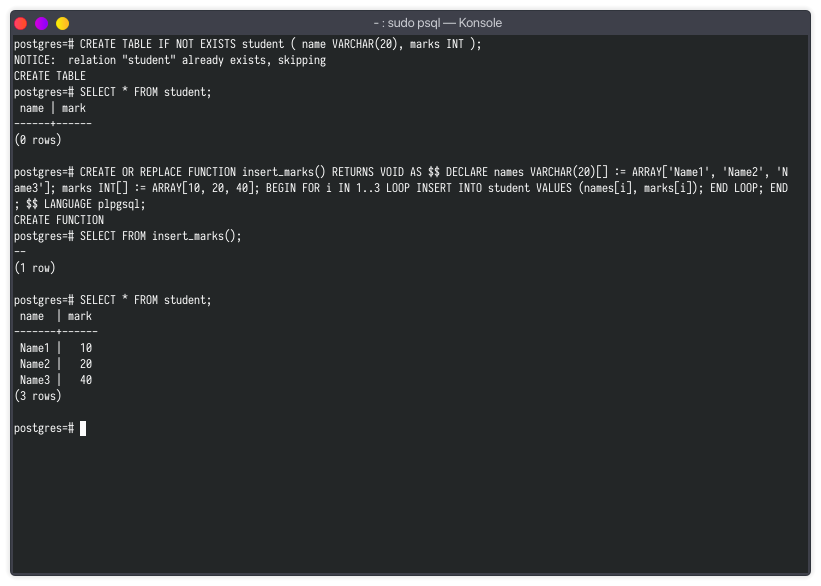
\includegraphics[width=0.9\textwidth]{img/p8/ss5.png}


\item
Create a sequence using PL/SQL. Use this sequence to generate the primary key
 values for a table named class\_cse with attributes roll, name and phone. Insert some
 tuples using PL/SQL programming.
Syntax:
\begin{verbatim}
CREATE TABLE IF NOT EXISTS class_cse (
        roll INT PRIMARY KEY,
        name VARCHAR(20),
        phone VARCHAR(15)
);
CREATE SEQUENCE key
START 100;
CREATE OR REPLACE FUNCTION class_cse_insert (
        name VARCHAR(20),
        phone VARCHAR(15)
) RETURNS VOID AS $$
BEGIN
        INSERT INTO class_cse VALUES 
                (NEXTVAL('key'), name, phone);
END;
$$ LANGUAGE plpgsql;
\end{verbatim}
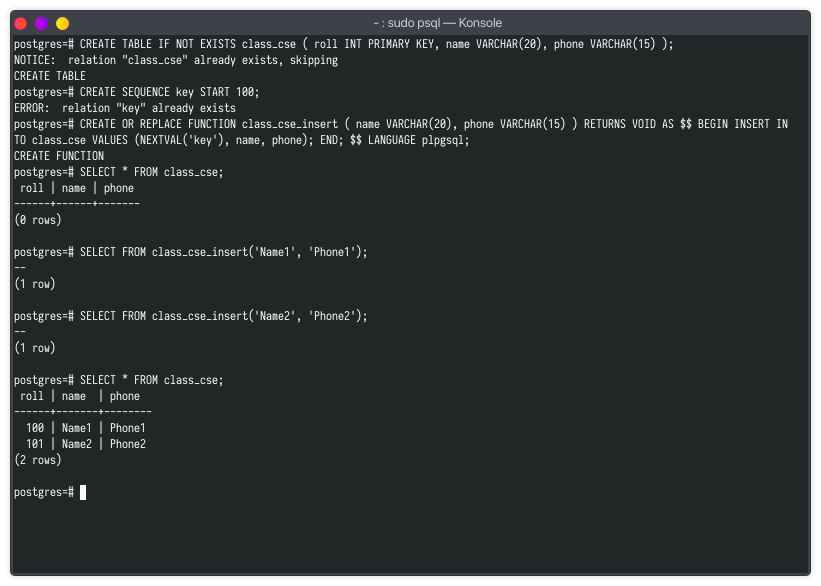
\includegraphics[width=0.9\textwidth]{img/p8/ss6.png}
	
\end{itemize}
\section*{Result}
	The PL/pgSQL functions are executed and their result
	is verified in a PostgreSQL environment.
\end{document} 